
                \begin{figure}
                    \centering
                    \begin{tikzpicture}
                        \pgfplotsset{%
                            width=1\textwidth,
                            height=0.5\textheight
                        }
                        \begin{axis}[
                            xlabel={Start battery level},
                            ylabel={Average dynamic energy (watt)},
                            ymin=0,ymax=20,
                        ]
                        
                            \addplot [mark=none, ultra thick, red]  coordinates {
                            (40, 9.080317639771367)(45, 9.056028700892501)(50, 9.096503887014311)(55, 9.074241116694191)(60, 9.140123387128373)(65, 9.045692708379416)(70, 9.006755519218176)(75, 9.000236953864679)(80, 8.577650960792491)
                            };
                            \addlegendentry{Surface4Pro - IntelPowerGadget}
                            
                            \addplot [mark=none, ultra thick, blue]  coordinates {
                            (40, 8.866856788873834)(45, 8.939403215137155)(50, 8.878338892427502)(55, 8.93372087824597)(60, 8.901989175752718)(65, 8.936604655382432)(70, 8.93115572015441)(75, 8.862165122986847)(80, 8.567210711115008)
                            };
                            \addlegendentry{Surface4Pro - HardwareMonitor}
                            
                            \addplot [mark=none, ultra thick, orange]  coordinates {
                            (45, 7.84335155965295)(50, 7.8340217816761095)(55, 7.831861100897588)(60, 7.824605336289419)(65, 7.812431901476497)(70, 7.809147329991928)(75, 7.813903060498174)(80, 7.713118039033552)
                            };
                            \addlegendentry{Surface4Pro - RAPL}
                            
                            \addplot [mark=none, dashdotted, red]  coordinates {
                            (40, 2.232978782017787)(45, 2.275319559617722)(50, 2.1453799184538376)(55, 2.240227021462736)(60, 2.3666097904684684)(65, 2.3410247382691978)(70, 2.3966303778983655)(75, 2.4716321826073755)(80, 2.6098105900542294)
                            };
                            \addlegendentry{SurfaceBook - IntelPowerGadget}
                            
                            \addplot [mark=none, dashdotted, blue]  coordinates {
                            (40, 2.2683979954552673)(45, 2.41769515731139)(50, 2.307831009740579)(55, 2.231641761992374)(60, 2.246953534638232)(65, 2.2551271061892337)(70, 2.337371018206007)(75, 2.558624738973859)(80, 2.62842302428329)
                            };
                            \addlegendentry{SurfaceBook - HardwareMonitor}
                            
                            \addplot [mark=none, dashdotted, orange]  coordinates {
                            (40, 5.250525672559464)(45, 5.254438901315704)(50, 5.289685432185107)(55, 5.372767682779623)(60, 5.370435058492623)(65, 5.413690439854076)(70, 5.523236199326845)(75, 5.685597158819214)(80, 5.779161109708826)
                            };
                            \addlegendentry{SurfaceBook - RAPL}
                            
                        \end{axis}
                    \end{tikzpicture} 
                \caption{A graph illustrating the energy consumption of Cores for test case Fasta with regards to the battey level of the DUT (with outliers)} \label{fig:Fasta_Cores_charge}
                \end{figure}
                